\documentclass[a4paper]{article}

%% Language and font encodings
\usepackage[english]{babel}
\usepackage[utf8x]{inputenc}
\usepackage[T1]{fontenc}
\usepackage{epigraph}
\usepackage{graphicx}
\usepackage{amsmath}
\usepackage{amsthm}
\usepackage{amstext} % for \text macro
\usepackage{array}   % for \newcolumntype macro
\usepackage{tabu}
\newcolumntype{R}{>{$}r<{$}} % math-mode version of ``l" column type

%% Sets page size and margins
\usepackage[a4paper,top=3cm,bottom=2cm,left=3cm,right=3cm,marginparwidth=1.75cm]{geometry}

%% Useful packages
\usepackage{amsmath}
\usepackage{graphicx}
%\usepackage{url}
\usepackage{hyperref}
\usepackage[colorinlistoftodos]{todonotes}
\usepackage{hyperref}
\usepackage{pgfplots}
\pgfplotsset{compat=1.9}

\usepackage{tikz}
\usetikzlibrary{decorations.pathmorphing,patterns}
\usetikzlibrary{external}
\tikzexternalize

\theoremstyle{definition}
\newtheorem{example}{Example}[section]

\title{Operator methods for integrals and differential equations}
\author{Dan Piponi}

\begin{document}
\maketitle

\epigraph{In memory of Tom Mower who started me on this journey more than three decades ago}

\begin{abstract}
Some techniques for abusing the operator $D=\frac{d}{dx}$ for both symbolic and numberic integration and differential equation solving.
Note: work in progress.
There are errors, some of which I know about.
Notation is also inconsistent.
\end{abstract}

\section{Warm up}
\subsection{A differential equation}
Suppose we are give the differential equation:
\[
\frac{df}{dx}+f = x^2
\]
Let's use the shorthand $D=\frac{d}{dx}$ and rewrite this as
\[
(D+1)f = x^2
\]
The standard approach is first to solve the homogeneous form of the equation
\[
(D+1)f = 0
\]
giving $f(x) = A\exp(-x)$ for some constant $A$.
We then have to find a \emph{particular integral}, i.e. any solution to the original equation.
The full solution to the original equation is the particular integral plus $A\exp(-x)$.

So how do we find a particular integral?
In my experience students are encouraged to use educated guesswork.
Anything goes as long as you prove that what you have found is indeed a solution.
So in this case a popular approach might be to assume $f(x)=Ax^2+Bx+C$, substitute into the equation, and solve for $A$, $B$ and $C$.

Here's a more direct way:
\begin{eqnarray*}
(D+1)f & = & x^2 \\
f      & = & \frac{1}{1+D}x^2 \\
       & = & (1-D+D^2+D^3-\ldots)x^2 \\
       & = & x^2-2x+2 \\
\end{eqnarray*}
We have performed two unusual operations:
\begin{enumerate}
\item we've ``divided'' by $1+D$ and
\item we've expanded $(1+D)^{-1}$ as a power series.
\end{enumerate}

\subsection{An integral}
Another example. Suppose we wish to find the integral:
\[
\int x^3\exp(2x) dx
\]
Integration is the ``inverse'' of differentiation so let's rewrite this as
\[
\frac{1}{D}x^3\exp(2x)
\]
Now we use a trick known as the shift rule. It states
\[
f(D)\exp(ax) = \exp(ax)f(D+a)
\]
So we can rewrite our integral as
\begin{eqnarray}
  & \exp(2x)\frac{1}{D+2}x^3 \\
= & \exp(2x)\frac{1}{2}\frac{1}{1+D/2}x^3 \\
= & \exp(2x)\frac{1}{2}(1-\frac{D}{2}+(\frac{D}{2})^2-(\frac{D}{2})^3+\ldots)x^3 \\
= & \frac{1}{2}\exp(2x)(x^3-\frac{3}{2}x^2+\frac{3}{2}x-\frac{3}{4}) \\
= & \frac{1}{8}\exp(2x)(4x^3-6x^2+6x-3) \\
\end{eqnarray}
We have used the same division and power series operations as above.
And of course for the full answer we need to add a constant $C$.

My goal here is to sketch (without full rigour) why you might expect such methods to work and give many more examples.
I also want to show how you can stretch these methods to give some hand-wavey arguments for some well-known theorems.

\section{Some justification}
\subsection{Truncated power series}
Let $P(x)$ be a polynomial in $x$.
Suppose we can expand $P(x)^{-1}$ as a power series with some non-empty circle of convergence:
\[
\frac{1}{P(x)} = \sum_{i=0}^\infty a_ix^i
\]
We have that
\[
P(x)\sum_{i=0}^\infty a_ix^i = 1
\]
so
\[
P(x)(\sum_{i=0}^{n-1} a_ix^i+\sum_{i=n}^\infty a_ix^i) = 1
\]
and
\[
P(x)\sum_{i=0}^{n-1} a_ix^i = 1-P(x)\sum_{i=n}^\infty a_ix^i
\]
The left hand side
\[
P(x)\sum_{i=0}^{n-1} a_ix^i
\]
is a polynomial.
It must be $1$ followed by terms of degree $n$ or higher.

For example
\begin{eqnarray*}
(1+x)(1-x+x^2-x^3+x^4) & = & 1-x+x^2-x^3+x^4-x^2+x^3-x^4+x^5 \\
                       & = & 1+x^5
\end{eqnarray*}

This tells us that we can use truncated power series to compute reciprocals of polynomials as long as we don't mind some higher order terms.
The nice thing about this is that we know that for any polynomial $Q(x)$, $D^nQ(x) = 0$ for $n$ large enough.
So we can use truncated power series in $D$ to obtain exact results when applied to polynomials in $x$.

Let me rewrite the first argument above in a more rigorous way:
\begin{eqnarray*}
(D+1)f & = & x^2 \\
(1-D+D^2)(D+1)f & = & (1-D+D^2)x^2 \\
     1f & = & x^2-2x+2 \mbox{ (assuming that $f$ has no terms beyond $x^2$)} \\
\end{eqnarray*}

We can see this as justifying the use of the operator $(D+1)^{-1}$ as long as we remember that the original argument is just a kind of shorthand for the rigorous one.

\subsection{The shift rule}
By the Leibniz rule we have
\begin{eqnarray*}
\frac{d}{dx}(\exp(ax)f(x)) & = & \exp(ax)\frac{df(x)}{dx}+a\exp(ax)f(x)
\end{eqnarray*}
We can rewrite this as
\begin{eqnarray*}
D(\exp(ax)f(x)) & = & \exp(ax)(Df(x)+af(x)) \\
                & = & \exp(ax)(D+a)f(x)
\end{eqnarray*}

We can write this even more compactly as
\[
D\exp(ax) = \exp(ax)(D+a)
\]
as long as we remember that in this version there is an implication that the $\exp(ax)$ on the left hand side is intended to be multiplied by some further expresion to its right.

We can prove more.
\begin{eqnarray*}
D^n\exp(ax) & = & D^{n-1}\exp(ax)(D+a) \\
            & = & D^{n-2}\exp(ax)(D+a)^2 \\
            & \vdots & \\
            & = & \exp(ax)(D+a)^n \\
\end{eqnarray*}
More generally we have The Shift Rule
\[
\boxed{f(D)\exp(ax) = \exp(ax)f(D+a)}
\]
for any polynomial $f$.
We also expect this to hold in situations where $f$ is a power series but we know it's being applied to a polynomial so terms beyond a certain point contribute zero.

\subsection{Integration again}
Now consider our integral above.
We can consider this as a solution to the differential equation
\[
Df = \exp(2x)x^3
\]
Using the shift rule we have
\begin{eqnarray*}
Df & = & \exp(2x)x^3 \\
\exp(2x)(D+2)\exp(-2x)f(x) & = & \exp(2x)x^2 \\
(D+2)\exp(-2x)f(x) & = & x^2 \\
\end{eqnarray*}
Writing $g(x) = \exp(-2x)f(x)$ we can now use the differential equation solving methods above to solve $(D+2)g = x^2$ and our final integral is given by $\exp(2x)g(x)$.
Again, we can see the original argument as being shorthand for this more rigorous argument.

\section{Diagonalisation}
The functions $\sin$, $\cos$ and $\exp$ ``diagonalise'' various differential operators.
This means that differential operators act on these functions just like multiplication by some number.
(That's what \emph{diagonalisation} means - finding elements that operators act on like real numbers.)
For example $D\exp(ax) = a\exp(ax)$.
But we also have $D^n\exp(ax) = a^n\exp(ax)$ and so
\[
f(D)\exp(ax) = f(a)\exp(ax)
\]
You can see this is a special case of the shift rule applied to $f(D)(\exp(ax)\times1)$.

We also have $D^2\sin(ax) = -a^2\sin(ax)$ and $D^2\cos(ax) = -a^2\cos(x)$.
So for any polynomial $f$
\begin{eqnarray*}
f(D^2)\sin(ax) & = & f(-a^2)\sin(ax) \mbox { and} \\
f(D^2)\cos(ax) & = & f(-a^2)\cos(ax).
\end{eqnarray*}

\begin{example}
Find a solution to
\[
\frac{d^2f}{dx^2}-3\frac{df}{dx}+2f = \exp(3x)
\]
Rewrite as
\[
(D^2-3D+2)f = \exp(3x)
\]
so
\begin{eqnarray*}
f(x) & = & (D^2-3D+2)^{-1}\exp(3x) \\
     & = & (3^2-3\times3+2)^{-1}\exp(3x) \\
     & = & \frac{1}{2}\exp(3x) \\
\end{eqnarray*}
\end{example}

\begin{example}
Find a solution to
\[
(D^2+1)f = \cos(2x)
\]
We have
\begin{eqnarray*}
f(x) & = & (D^2+1)^{-1}\cos(2x) \\
     & = & (-2^2+1)^{-1}\cos(2x) \\
     & = & -\frac{1}{3}\cos(2x) \\
\end{eqnarray*}
\end{example}

\section{Lots of examples}
\begin{example}
Find a solution to
\[
\frac{df}{dx}+f = \sin x
\]
Unfortunately we have an odd power of $D$ applied to the $\sin$ function so we can't directly use the diagonalisation technique.
Instead we write $\sin x$ using Euler's formula:
\begin{eqnarray*}
\frac{1}{1+D}\sin x & = & \frac{1}{1+D}\Im(\exp{ix}) \\
                    & = & \Im\big(\frac{1}{1+D}\exp{ix}\big) \mbox{ (using fact that $\Im(D(f)) = D(\Im(f))$)} \\
                    & = & \Im\big(\frac{1}{1+i}\exp{ix}\big) \mbox{ (using diagonalisation for $\exp$)} \\
                    & = & \Im\big(\frac{1-i}{2}\exp{ix}\big) \\
                    & = & \frac{1}{2}(\sin x-\cos x) \\
\end{eqnarray*}
\end{example}

\begin{example}
Find a solution to
\[
\frac{d^3f}{dx^3}-f = \sin x
\]
We want
\[
\frac{-1}{1-D^3}\sin x
\]
We can use the fact that $D^2\sin x = -\sin x$ to reduce this to:
\[
\frac{-1}{1+D}\sin x
\]
The solution is just minus the previous example
\[
f(x) = \frac{1}{2}(\cos x-\sin x)
\]
\end{example}

\begin{example}
Find a solution to
\[
\frac{d^2f}{dx^2}-2\frac{df}{dx}+f=e^x
\]
The only slight subtlety here is noticing that when we use the shift rule, we slide $f(D)$ past $\exp x$ leaving behind a 1 that needs to be integrated twice.
\begin{eqnarray*}
(D^2-2D+1)f & = & e^x \\
f & = & \frac{1}{(D-1)^2} e^x \\
  & = & e^x\frac{1}{D^2}1 \\
  & = & \frac{x^2}{2}e^x
\end{eqnarray*}
\end{example}

\begin{example}
Find a solution to
\[
4\frac{d^2f}{dx^2}+f = x\exp(-x)
\]
Solution:
\begin{eqnarray*}
\frac{1}{1+4D^2}\exp(-x)x & = & \exp(-x)\frac{1}{1+4(D-1)^2}x \\
& = & \exp(-x)\frac{1}{4D^2-8D+5}x \\
& = & \frac{1}{5}\exp(-x)\frac{1}{1-8D/5}x \mbox{ (using $D^2x=0$)}\\
& = & \frac{1}{5}\exp(-x)(1+\frac{8}{5}D)x \\
& = & \frac{1}{25}\exp(-x)(5x+8) \\
\end{eqnarray*}

\end{example}

\begin{example}
Find
\[
\int_0^\infty x^n\exp(-x)dx
\]
First the indefinite integral
\begin{eqnarray*}
&   & \frac{1}{D}x^n\exp(-x) \\
& = & \exp(-x)\frac{1}{D-1}x^n \\
& = & -\exp(-x)(1+D+D^2+\ldots+D^n)x^n \\
\end{eqnarray*}
We're going to be evaluating this at zero and in the limit as $x$ goes to infinity.
All of these terms vanish at infinity.
All of the non-constant derivatives of $x^n$ vanish at zero.
So we're left with
\[
\Big[-\exp(-x)D^nx^n\Big]_0^\infty
\]
This is $n!$.
\end{example}

\begin{figure}
\centering
\frame{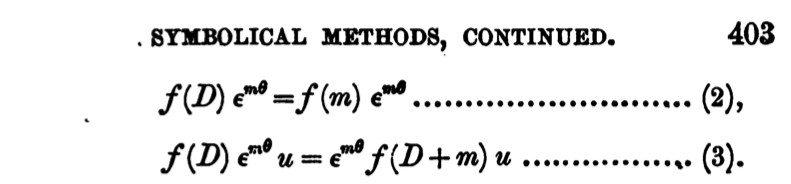
\includegraphics[width=5in]{shift2.png}}
\caption{These techniques are old. This snippet is from Boole's Treatise on Differential Equations from 1859.}
\end{figure}

\section{Exponentials of $D$}
Taylor's theorem tells us that
\[
f(x+a) = f(x)+af'(x)+\frac{a^2}{2!}f''(x)+\frac{a^3}{3!}f^{(3)}(x)+\ldots+\frac{a^n}{n!}f^{(n)}(x)+\mbox{ a remainder term}
\]
The form of the remainder depends on the class of function $f$.
For polynomials the remainder is precisely zero for $n$ large enough.
For analytic functions the remainder goes to zero as $n$ goes to infinity so we can write
\[
f(x+a) = \sum_{n=0}^\infty a^n\frac{D^n}{n!}(f)(x)
\]
We can now write this as
\[
f(x+a) = (\sum_{n=0}^\infty a^n\frac{D^n}{n!})(f)(x)
\]
and therefore as
\[
f(x+a) = \exp(aD)(f)(x)
\]
In other words, $\exp(aD)$ is the operator that shifts a function by $a$.

\section{Sums}
Armed with exponentials of $D$ we can extend our methods for integrals and differential equations to sums and recurrence relations.
\begin{example}
Find
\[
\sum_{x=0}^{n-1}x^3
\]
Write $f(x) = \sum_{y=0}^{x-1}y^3$.
Then we want to solve
\[
f(x+1)-f(x) = x^3
\]
\end{example}
We can now use the methods above:
\begin{eqnarray*}
\exp(D)f-f & = & x^3 \\
(\exp(D)-1)f & = & x^3 \\
f & = & \frac{1}{\exp(D)-1}x^3 \\
f & = & \frac{1}{D+\frac{1}{2}D^2+\frac{1}{3!}D^3+\frac{1}{4!}D^4+\frac{1}{5!}D^5}x^3 \\
f & = & \frac{1}{1+\frac{1}{2}D+\frac{1}{3!}D^2+\frac{1}{4!}D^3+\frac{1}{5!}D^4}\int x^3dx \\
f & = & \frac{1}{1+\frac{1}{2}D+\frac{1}{3!}D^2+\frac{1}{4!}D^3+\frac{1}{5!}D^4}\frac{1}{4}x^4 \\
\end{eqnarray*}
There are tricks we can use to minimise the work here although I'm going to be a bit more explicit than needed so everything is clear.
Analogously to solving differential equations, we are going to end up with a ``particular sum''.
The full solution is going to require determining a constant term.
But it's clear that the sum needs to be zero for $x=0$ so the constant term should be zero.
Applying $D^4$ to $x^4$ is going to give us a constant term.
So we only need to keep terms up to $D^3$.
We get
\begin{eqnarray*}
f & = & \frac{1}{4}(1-(\frac{1}{2}D+\frac{1}{3!}D^2+\frac{1}{4!}D^3)+
        (\frac{1}{2}D+\frac{1}{3!}D^2)^2-(\frac{1}{2}D)^3)x^4 \\
  & = & \frac{1}{4}(1-\frac{1}{2}D-\frac{1}{6}D^2-\frac{1}{24}D^3+
        \frac{1}{4}D^2+\frac{1}{6}D^3-\frac{1}{8}D^3)x^4 \\
  & = & \frac{1}{4}(1-\frac{1}{2}D+\frac{1}{12}D^2)x^4 \mbox{ (nice for us, the cubic term vanishes)} \\
  & = & \frac{x^4}{4}-\frac{x^3}{2}+\frac{x^2}{4} \\
\end{eqnarray*}
This may seem borderline magical.
One way to think about it is that if we know $f$ is a degree 4 polynomial, then $f(x+1) = f(x)+f'(x)+\frac{1}{2}f''(x)+\frac{1}{3!}f^{(3)}(x)+\frac{1}{4!}f^{(4)}(x)$ exactly.
So solving the summation is equivalent to solving the differential equation
\[
\frac{1}{4!}\frac{d^4f}{dx^4}+\frac{1}{3!}\frac{d^3f}{dx^3}+\frac{1}{2}\frac{d^2f}{dx^2}+\frac{df}{dx} = x^3
\]
It is entirely reasonable to solve this using differential equation methods.
If you extend this approach beyond polynomials you rediscover the Euler-Maclaurin summation formula.

\begin{example}
Solve
\[
a_{n+2}=a_{n+1}+a_n+n^2 \mbox{ with } a_0=0, a_1=0
\]
In this case the problem requires finding a spolution with specific initial conditions.
So we're going to need both a ``particular sum'' and a solution to the homogeneous equation.
It's well known that the solutions to the homogeneous equation are the Fibonacci numbers $F_n$ and the Lucas numbers $L_n$.
Any other solution is a linear combination of these.
The Fibonacci numbers start with $F_0=0$ and $F_1=1$ and the Lucas numbers start with $L_0=2$ and $L_1=1$.

Let's write $a_x=f(x)+AF_x+BL_x$ so our notation matches what used earlier.
We have
\begin{eqnarray*}
(e^{2D}-e^D-1)f & = & x^2 \\
f & = & \frac{1}{e^{2D}-e^D-1}x^2 \\
  & = & (-1-D-\frac{5}{2}D^2)x^2 \\
  & = & -x^2-2x-5
\end{eqnarray*}
Because $F_0=0$, the initial condition at $x=0$ immediately implies that $B$ is $\frac{5}{L_0}=\frac{5}{2}$.
The initial condition at $x=1$ now gives $A=\frac{11}{2}$.
The complete solution is
\[
a_n = \frac{5}{2}L_n+\frac{11}{2}F_n-n^2-2n-5
\]
By the way, Mathematica makes a real mess of this.
\end{example}

\section{Numerical methods}
\subsection{Derivatives}
The relation $(e^{hD}-1)f(x) = f(x+h)-f(x)$ expresses a finite difference in terms of the differential operator.
We can do this in reverse and derive formulae for derivatives in terms of finite differences.
A good application of this is to derive approximations of derivatives that we can use in numerical methods on a grid.
Define $E_h = e^{hD}$. We'd like to write $D$ in terms of $E_h$.
That seems straightforward. We expect
\[
D=\frac{1}{h}\log E_h
\]

The problem is, we can't simply apply a Taylor expansion to $\log E_h$ about $0$.
Suppose we'd like our numerical methods to work well on polynomials - typically giving exact results on low order polynomials.
The operator $E_h-1$ corresponds to finite differencing and we know that repeated finite differences applied to polynomials eventually give zero.
So if we seek a power series in $E_h-1$ we can guarantee convergence on polynomials.
Let's define the finite difference operator $\Delta_h = e^{hD}-1 = E_h-1$.
So we should expand $\log E_h$ around $1$ and use
\[
D = \log(1+(E_h-1))
\]

Let's try a first order expansion.
We get
\[
\log(1+(E_h-1)) = E_h-1 + \mbox{higher order terms} 
\]
In other words we can approximate the derivative of $f$ with
\[
f'(x) \approx \frac{f(x+h)-f(x)}{h}
\]
As we might expect, this is exact if $f$ is a linear function.
What if we try second order.
\begin{eqnarray*}
\log(1+(E_h-1)) & \approx  & E_h-1 - \frac{1}{2}(E_h-1)^2 \\
& = & -\frac{1}{2}E_h^2+2E_h-\frac{3}{2}
\end{eqnarray*}
So we get
\[
f'(x) \approx \frac{-f(x+2h)+4f(x+h)-3f(x)}{2h}
\]
This is known as a second-order upwind scheme.
It's ``upwind'' because it's using values of $f$ on one side of $x$ to estimate the derivative.
This is good in numerical methods where you only want to look at one side - for example in simulations of convection where we're trying to estimate what happens in the future and so shouldn't be using information corresponding to fluid that has already come and gone.
But often we want a balanced estimate of the derivative.
But a power series in $e^{hD}$ can't ever refer to points left of $x$.
On the other hand we could try to estimate $f'(x+h)$.
In other words, we should compute $E_hD=e^{hD}D$ in terms of $E_h$.
Clearly
\[
E_hD = E_h\log E_h
\]
Expanding around $1$ we get
\begin{eqnarray*}
E_hD & = & (1+\Delta_h)\log(1+\Delta_h) \\
& \approx & (1+\Delta_h)(\Delta_h-\frac{1}{2}\Delta_h^2) \\
& \approx & \Delta_h+\frac{1}{2}\Delta_h^2 \\
& = & E_h-1+\frac{1}{2}(E_h-1)^2 \\
& = & -\frac{1}{2}+\frac{1}{2}E_h^2\\
\end{eqnarray*}
So $f'(x+h) \approx \frac{1}{h}(f(x+2h)-x(f))$ or
\[
f'(x) \approx \frac{f(x+h)-f(x-h)}{2h}.
\]
which is the usual central difference formula.

More generally, we can use the power series of $\Delta_h^m\log\Delta_h$ up to terms in $\Delta_h^k$ to generate an $k$th order estimate for $D$.
Even more generally, we can use the power series of $\Delta_h^m(\log\Delta_h)^n$ to estimate $D^n$.

\begin{example}
Derive a 3rd order upwind estimate for $D$ using $f(x-h),\ldots,f(x+3h)$.
Solution:
\begin{eqnarray*}
(1+\Delta_h)\log(1+\Delta_h) & \approx & (1+\Delta_h)(\Delta_h-\frac{1}{2}\Delta_h^2+\frac{1}{3}\Delta_h^3) \\
& = & \Delta_h-\frac{1}{2}\Delta_h^2+\frac{1}{3}\Delta_h^3+\Delta_h^2-\frac{1}{2}\Delta_h^3 \\
& = & \Delta_h+\frac{1}{2}\Delta_h^2-\frac{1}{6}\Delta_h^3 \\
& = & E_h-1+\frac{1}{2}(E_h-1)^2-\frac{1}{6}(E_h-1)^3 \\
& = & E_h-1+\frac{1}{2}(E_h^2-2E_h+1)-\frac{1}{6}(E_h^3-3E_h^2+3E_h-1) \\
& = & -\frac{1}{3}-\frac{1}{2}E_h+E_h^2-\frac{1}{6}E_h^3 \\
\end{eqnarray*}
So 
\[
f'(x) = \frac{-2f(x-h)-3f(x)+6f(x+h)-f(x+2h)}{6}
\]
\end{example}

\begin{example}
Derive a symmetric 4th order order estimate for the third drivative.
Solution:
\begin{eqnarray*}
(1+\Delta_h)^2(\log(1+\Delta_h))^3 & \approx &
(1+\Delta_h)^2(\Delta_h-\frac{1}{2}\Delta_h^2+\frac{1}{3}\Delta_h^3-\frac{1}{4}\Delta_h^4)^2 \\
& \approx & \Delta_h^3+\frac{1}{2}\Delta_h^4 \\
& = & \frac{1}{2}(-1+2\Delta_h^2-2\Delta_h^2+\Delta_h^3) \\
\end{eqnarray*}
So
\[
f^{(3)}(x) \approx \frac{-f(x-2h)+2f(x-h)-2f(x+h)+f(x+2h)}{2}
\]
\end{example}

\subsection{A generating function for all one-sided derivative schemes}
Suppose we have a power series $f(x) = a_0+a_1x+a_2x^2+\ldots$.
We can form a generating function for the $n$th partial sum $a_0+a_1x+\ldots+a_{n-1}x^{n-1}$ as
\[
a_0+k(a_0+a_1x)+k^2(a_0+a_1x+a_2x^2)+\ldots
\]
Assuming absolute convergence can rearrange this as
\begin{eqnarray*}
& & (1+k+k^2+\ldots)a_0
+k(1+k+k^2+\ldots)a_1x
+k^2(1+k+k^2+\ldots)a_2x^2+\ldots \\
& = & \frac{1}{1-k}(a_0+a_1(kx)+a_2(kx)^2+\ldots) \\
& = & f(kx)/(1-k)
\end{eqnarray*}
The $n$th order one-sided derivative is derived using $n$ terms from $\log E_h = \log(1+\Delta_h)$.
So the coefficients from the $n$th order scheme are the coefficients of the polynomial in $x$ that forms the coefficient of $k^n$ in $\frac{\log(1+(x-1)k)}{1-k}$.
We can tabulate this as
\begin{center}
\tabulinesep=1.2mm
\begin{tabu}{|c| R  R  R  R  R  R  R  R|}
\hline
\text{Order} & \multicolumn{8}{| l |}{Coefficients} \\
\hline
0 & 0 & & & & & & & \\
1 & -1 & 1 & & & & & & \\
2 & \frac{-3}{2} & 2 & \frac{-1}{2} & & & & & \\
3 & \frac{-11}{6} & 3 & \frac{-3}{2} & \frac{1}{3} & & & & \\
4 & \frac{-25}{12} & 4 & -3 & \frac{4}{3} & \frac{-1}{4} & & & \\
5 & \frac{-137}{60} & 5 & -5 & \frac{10}{3} & \frac{-5}{4} & \frac{1}{5} & & \\
\hline
\end{tabu}
\end{center}
This reproduces the table in \cite{Fornberg1988}.
All of the results in that paper can be reproduced by forming power series from expressions of the form $(1+x)^m(\log(1+x))^n$, with $m$ a half-integer in some cases.

Incidentally, I used the second order scheme from this table in ILM's GPU based fluid simulator basing my work on \cite{SCA:SCA08:009-018}.
I derived it using the techniques described above but it disagreed with the paper.
It turned out that the paper had an error.
The moral is: it's worth knowing how to derive these schemes even if they appear to be available already in publications.

\subsection{Caveat}
Before using any of these methods in any kind of differential equation solver please consider doing a von Neumann stability analysis.
It's sometimes hard to guess which methods are and aren't stable.

\subsection{Numerical Integration}
We can write
\[
\int_a^b f(x)dx = \Big(\frac{e^{bD}-e^{aD}}{D}f\Big)(0)
\]
There are two ways to see this.
One is to view $\frac{1}{D}f$ as the indefinite integral with $e^{bD}$ and $e^{aD}$ picking out the value of this indefinite integral at $x=b$ and $x=a$.
Another is the following derivation:
\begin{eqnarray*}
\int_a^b f(x)dx & = & \Big(\int_a^b\exp(yD)f\Big)(0) dy \\
& = & \Big(\int_a^b\exp(yD)dy f\Big)(0) \\
& = & \Big(\frac{e^{bD}-e^{aD}}{D}f\Big)(0) \\
\end{eqnarray*}
if you can make yourself to believe that $D$ can behave like an ordinary number in an integration.
This means we can expect to derive useful integration schemes using

\subsection{Simpson's rule}

\subsection{Newton-Coates rules}

\subsection{Bessel functions and integrating oover disks}

\bibliographystyle{unsrt}
\bibliography{operators}

\end{document}
